\section{Genetischer Algorithmus}
\label{Sec:GeneticAlgorithmDetail}
\subsection{Suchproblem Formalisierung}
Um einen genetischen Algorithmus für ein Problem sinnvoll zu verwenden, muss zuerst einmal ein zugrunde liegendes Problem als Suchproblem formuliert werden. Im vorliegenden Anwendungsfall würde eine solche Formalisierung daraus bestehen.
    

Sei $K = \{e_1, e_2, \ldots, e_n\}$ eine Menge von Elementen, wobei jedes Element $e_i$ entweder vom Typ $O$ oder $E$ ist. Gesucht ist eine Konfiguration $K$, sodass die Funktion $f(K)$ maximiert wird.

Der vorhandene genetische Algorithmus wurde auf Basis des vorliegenden Problems mit 2 Obfuskatoren entwickelt und dafür optimiert. Die vorgestellten Obfuskatoren sind dabei als Beispiele für ein Array von verschiedenen Verschleierungsmöglichkeiten und Technologien zu verstehen, die in Kombination eingesetzt werden könnten. Einige Entscheidungen für spezifische genetische Operatoren wurden mittels eines Pretests getroffen \ref{methode:pretest}.

\subsection{Fitness Funktion}
Die Fitness Funktion setzt sich aus mehreren Faktoren zusammen und lässt sich nicht einfach als richtig oder falsch definieren sondern basiert stark auf dem zugrundeliegenden Optimierungsproblem. Das vorliegende Beispiel geht etwas über das Problem von klassischen genetischen Algorithmen hinaus, indem es nicht nur die Kandidaten optimieren soll, sondern zeitgleich auch noch die Laufzeit des gesamten Algorithmus möglichst kurz halten (Hyperparameter).
In diesem Fall gibt es die folgenden Faktoren:

    \subsubsection{Obfuskations und Detektions-Dauer}
    Wie lange braucht es die die obfuskierte Malware in all ihren Schritten zu erzeugen unter Verwendung von Cashing. Dies ist einer der genannten Hyperparameter, da die gesamte Laufzeit des Algorithmus sich aus der Summe von durchgeführten Obfuskations und Detektionszeiten zusammensetzt und eine Population, die aus Kandidaten besteht, die nur kurze Obfuskations und Detektionsdauern hat, zu einer kürzeren Laufzeit beiträgt. $t_O,  t_D$
    
    \subsubsection{Obfuskationsschritte}
    Die Anzahl an Obfuskationsschritten, die der Kandidat behinhaltet. Dies hängt auch stark mit der initalen Population von Kandidaten zusammen und wie häufig diese gestapelt sind \ref{GA:inital_population}. $N_O$
    
    \subsubsection{Detektionsergebnis}
    Die Ergebnisse des Scanners, ob die Datei als Malware erkannt wurde und ob der Scanner sie überhaupt durchführen konnte und damit lauffähig ist. $D_{Malicious}=1, D_{Benign}=10^5$
    
    \subsubsection{Funktion}
    Die Funktion zeichnet sich durch die oben genannten Hyperparameter aus. Diese sollen zwar nicht für die einzelnen Kandidaten entscheidend sein, dennoch einen Einfluss auf die Gesamtheit der Population haben.
    Der Primäre Zweck der Funktion ist es, Malware so zu obfuskieren, dass sie nicht erkannt wird. Sekundär soll dabei die Laufzeit des gesamten Algorithmus klein gehalten werden. Dies kann zu einem Teil durch die Fitnessfunktion bewerkstelligt werden, zum anderen über Caching, welches durch die Fitnessfunktion belohnt werden soll. Andererseits soll für die Analyse der wissenschaftlichen Fragestellung die Verwendung von mehrstufigen Obfuskationen befürwortet werden. Eine Möglichkeit dies zu gewährleisten ist es, dass man die Obfuskationszeit von gecachten nicht künstlich erhöht und nachhält, sondern nur die tatsächlich verbrauchte Zeit bis zum fertig obfuskierten Payload gemessen wird und als $t_O$ interpretiert wird.
    Ein weiterer Ansatz, um das Gleichgewicht zwischen Minimierung von Laufzeit und Diversität der Lösungslängen zu wahren, wäre eine T/Z-Transformation der Obfuskationszeiten mit einer angenommenen $\sigma _{t_D}=5s$ und $\overline{M_{t_D}}$
    $\frac{D_{Benign, Malicious}}{t_D}+t_O$
\subsection{Encoding}
Die Lösungskandidaten bestehen aus einer Liste von Obfuskator Konfigurationen. Diese Obfuskatorkonfigurationen beinhalten jeweils alle Eigenschaften, die für jeden der Obfuskatoren als Optionen nötig sind, und benutzen die Eigenschaften, die für den ausgewählten Obfuskator nötig sind. Dies hat zwar zur Folge, dass es starke epigenetische Effekte\footnote{Veränderung eines Genes, die kaskadierende Auswirkungen auf die restlichen Gene im Kandidaten hat} geben und Mutationen völlig ergebnislos bleiben, ermöglicht dafür aber die sinnvolle Verwendung von diversen Rekombinationsarten. Konzeptionell besteht das Encoding damit also aus einem String von gequantelter Größe, die allerdings nicht konstant ist. 
In genetischen Algorithmen ist es eher ungewöhnlich, dass die Länge eines Lösungskandidaten ungleich der von anderen ist, was bei der Rekombination zu Problemen geführt hat. Die Entscheidung für dieses Design liegt darin, dass der Algorithmus von selbst die optimale Obfuskationslänge entscheiden soll und zeitgleich möglichst laufzeiteffizient werden soll.
\begin{figure}[h]
    \centering
    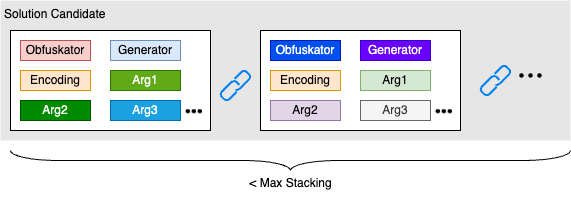
\includegraphics[width=0.85\textwidth]{gfx/Abbildungen/Encoding Diagram.png}
    \caption{Encoding Darstellung}
    \label{fig:encoding}
\end{figure}

\subsection{Selektion}
Für die Selektion wurde im Algorithmus auf die sogenannte Turnierselektion zurückgegriffen, die neben der einfachen Programmierbarkeit es auch leicht macht, den Selektionsdruck anzupassen. \cite{blickle_1996_a} (1995 Tournament Selection and Noise). Ein weiterer Vorteil dieses Verfahrens ist es, dass man nicht die Fitness aller mutierten und rekombinierten Kandidaten einer Population berechnen muss, sondern nur derjenigen, die in einem Turnier teilnehmen. Als weitere Ergänzung und Laufzeitoptimierung kommt der sogenannte "David"-Parameter zum Tragen, welcher dem unterlegenen Kandidaten in einem Turnier als Sieger hervorgehen lässt und so die Diversität der kommenden Generation erhöhen kann.

\subsection{Mutation}
\begin{figure}[h]
    \centering
    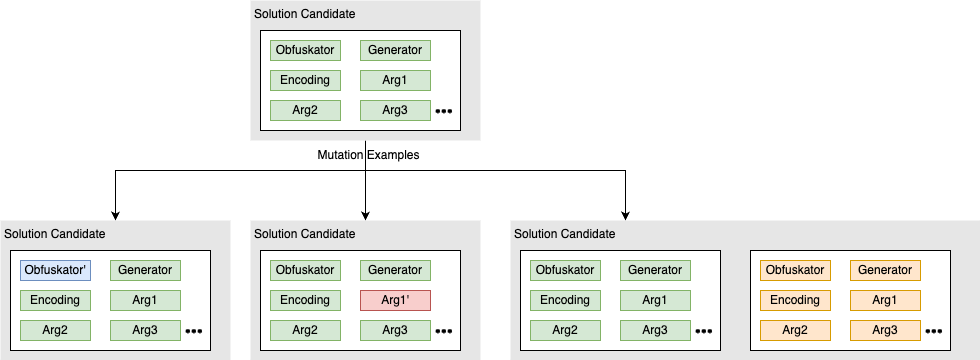
\includegraphics[width=0.85\textwidth]{gfx/Abbildungen/Mutations.png}
    \caption{Mutationsmöglichkeiten}
    \label{fig:mutations}
\end{figure}
Die Mutation ist in zwei Bestandteile aufgeteilt. Einerseits eine simple Veränderung einer Obfuskatorkonfiguration innerhalb des Lösungskandidaten und damit innerhalb der Liste. Andererseits das Hinzufügen von einer zufälligen neuen Obfuskatorkonfiguration in den Lösungskandidaten, um so eine längere Lösung zugänglich zu machen.


\subsection{Rekombination}
Für die Rekombination sind viele verschiedene Implementierungen möglich gewesen. Nach einigen Überlegungen wurden dann zwei verschiedene Rekombinationsarten implementiert und ausprobiert.
\subsubsection{String-based-Recombination}
Ähnlich dem klassischen Binary-String Encoding werden hier die Lösungskandidaten an einer beliebigen Stelle durchgeschnitten und die zweite Hälfte zwischen diesen ausgetasucht. Dieser Schnitt kann selbstverständlich an einer Obfuskationskonfigurationsgrenze auftreten und so nur das Stapeln verändert, aber auch innerhalb der Konfiguration.
\subsubsection{Sacrifice Based Shema}
In diesem Beispiel wird von einem Kandidaten eine Konfiguration entfernt und dem anderen Kandidaten hinzugefügt. Dies kann dazu führen, dass eine Lösung keine Obfuskationsschritte beinhaltet und dabei dann als nicht obfuskiertes File behandelt und gescanned wird.




\subsection{Startpopulation} \label{GA:inital_population}
Anhand von einigen Versuchen hat sich gezeigt, dass die gängige Praxis von genetischen Algorithmen, eine Populationsgröße von 100 oder größer zu wählen, den Effekt hat, dass die erste Generation eine fast vollständige Auflistung aller Einstelliger Obfuskatorkonfigurationen beinhaltet und somit keinen Vorteil gegenüber einer exhaustive search hat. Aus diesem Grund wurde ein Pretest angesetzt, um Laufzeitverhalten und Diversität innerhalb der Population in Abhängigkeit von verschiedenen Startpopulationsansätzen zu überprüfen und den Vorteil aus dem genetischen Algorithmus zu maximieren.
Deshalb und um \ref{Methode:Kriterien} zu befriedigen, wurde mit der standardmäßigen Populationszahl experimentiert, um den Vorteil von GAs gegenüber einem naiven durchprobieren hervorstechen zu lassen und gleichzeitig eine höhere Dichte von Lösungen mit mehreren Obfuskationsschritten zu haben.
\begin{itemize}
    \item 45 Lösungskandidaten, die zufällig mittels eines Stackingparameters erstellt wurden (Aktuelle Lösung)
    \item 20 Lösungskandidaten, die alle mit maximaler Länge erstellt werden
    \item 20 Lösungskandidaten, die zufällig mittels eines Stackingparameters erstellt wurden
\end{itemize}
\subsubsection{Aufbau Pretest}
Jede Konfiguration wurde mit Bening und Malware einmal durchgeführt und der Verlauf von Rechenzeit, also die Diversität und das Explorations vs Exploitverhalten betrachtet. Ziel ist es, dass die Rechenzeit nicht zu mehr als 80\% in der ersten Generation liegt.
\subsubsection{Ergebnisse}
\begin{table}[]
\begin{tabular}{@{}llll@{}}
\toprule
              & Shell        & Calc & Benign \\ \midrule
45 Random     & 423          & 384  & 621    \\
20 Random     & \textit{180} & 216  & 217    \\
20 Max Length & \textit{196} & \textit{211}  & 209    \\ \bottomrule
\end{tabular}
\caption{Runtimes for different Malware with different starting populations in seconds. Italic means unsucsessfull run}
\label{Pretest_Inital}
\end{table}
Im Pretest hat sich gezeigt, dass die Laufzeit mit der Anzahl zusammenhängt \ref{Pretest_Inital}. In einigen Fällen wurde überhaupt keine Lösung für das Problem gefunden, um die Scanner zu umgehen, diese Lösungen (20-Max-Length und 20-Random für Shell) fallen gänzlich aus dem Test heraus, da sie die grundlegende Funktionalität nicht erfüllen können.

Damit scheiden die Lösungen mit 20 Kandidaten gänzlich aus und wir verbleiben mit der Option von 45 zufälligen Kandidaten mit einem Stackingparamter <1.0.
